% Skrivet av Nils

Primtal är förrädiskt oförutsägbara.
De dyker upp när du minst anar det och kan till synes bete sig helt oregelbundet.
Trots detta är de helt deterministiska i sin natur och gränsen för vad som är och inte är ett primtal är mycket tydlig.
Det är kanske just av denna anledning som primtalen har fascinerat matematiker i tusentals år och fortsätter att göra så än idag.

Hur många primtal finns det? Svaret är att det finns oändligt många.
Om vi istället frågar oss hur många primtal det finns som är mindre än en miljon, så är svaret inte lika lätt.
Förutom talet 2 så är primtal aldrig jämna så vi kan åtminstone utesluta vartannat tal och säga att svaret är mindre än en halv miljon.
Hur går vi vidare härifrån?
Ett naturligt andra steg vore att föra samma resonemang för talet 3;
förutom just 3 så är primtal aldrig delbara med 3 så vi borde kunna dra bort ytterligare en tredjedels miljon från svaret.
Detta är dessvärre inte riktigt sant.
Tal som både är jämna och delbara med 3 har ju uteslutits två gånger.
Det har alltså skett en dubbelräkning av alla tal som kan delas med 6 men vi kan kompensera för detta genom att addera en sjättedels miljon till svaret.

Detta är en bättre uppskattning än vad vi hade tidigare och vi skulle givetvis kunna fortsätta med talet 5 och på så sätt komma ännu närmre det faktiska svaret.
Den generella idén kallas för \textit{inklusions-exklusionsprincipen} och illustreras nedan för tre mängder.
\begin{figure}[H]
    \centering
    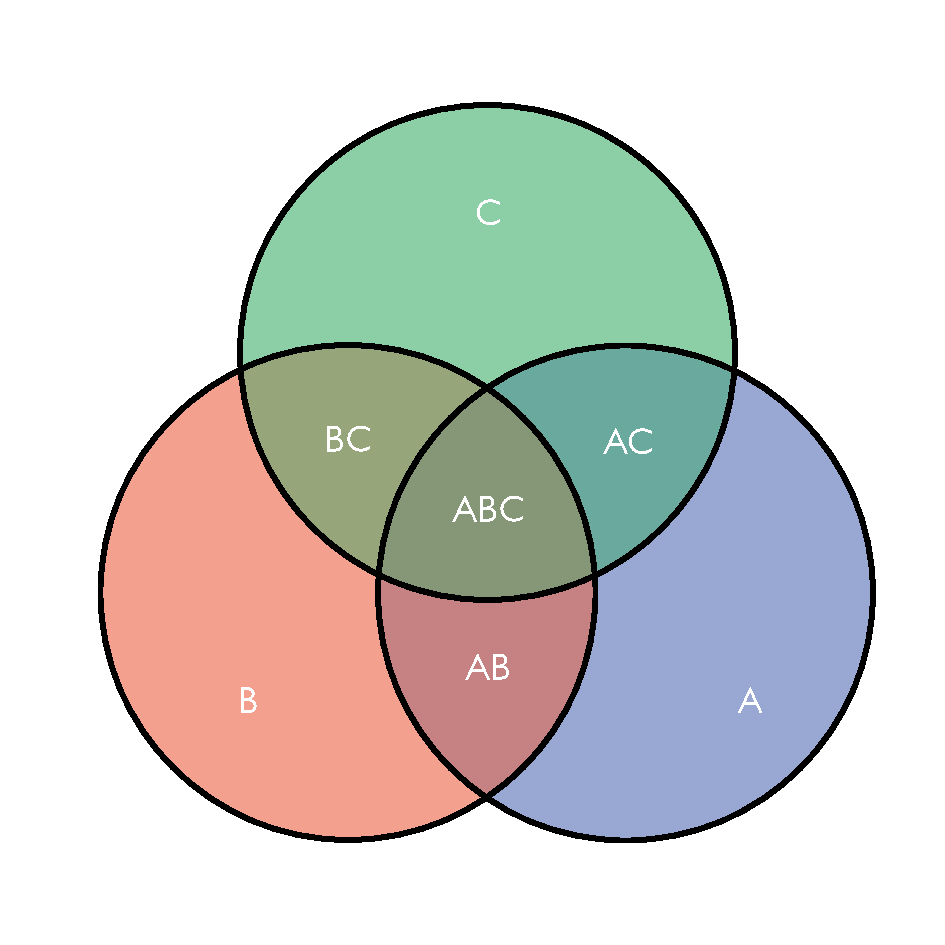
\includegraphics[scale=0.3]{erik/Images/Venndiagram.pdf}
\end{figure}
Säg att vi vill uppskatta den totala storleken de överlappande mängderna $A$, $B$ och $C$. 
Vi kan börja med att summera storleken på mängderna var för sig.
Om vi betecknar storleken på $A$ som $|A|$ och gör samma sak för de andra mängderna så kan vi skriva summan som $|A|+|B|+|C|$.
Men nu har det som bekant skett en dubbelräkning av överlappen $AB$, $BC$ samt $AC$, vi drar bort dessa från summan och får $|A|+|B|+|C|-|AB|-|BC|-|AC|$.
Dessutom har vi $ABC$ där alla tre mängder överlappar varandra.
Denna ingår i alla tidigare nämnda mängder och har därmed lagts till och dragits bort tre gånger om. 
Vi lägger till $ABC$ en gång till och kommer fram till svaret
\begin{equation*}
    |A|+|B|+|C|-|AB|-|BC|-|AC|+|ABC|.
\end{equation*}
Detta är inklusions-exklusionsprincipen och kan användas för godtyckligt många mängder.
Metoden att använda denna princip för att räkna primtal kallas för Legendres såll och är fundamental i teorin om matematiska såll.


Ett (matematiskt) såll är i stora drag en metod för att rensa bort vissa tal ur en större mängd.
Exempelvis som ovan när vi använde Legendres såll för att utesluta tal som inte är primtal ur mängden av heltal upp till en miljon.
I denna rapport kommer vi att presentera tre stycken såll; Eratosthenes generaliserade såll, Bruns såll samt Selbergs såll som alla bygger på liknande idéer som ovanstående.










\begin{comment}
Dubbelräkningen skedde eftersom vi hade två stycken mängder av tal som överlappade varandra och vi kompenserade genom att återlägga överlappet.

Denna idé kallas för \textit{inklusions-exklusionsprincipen} och kan även användas när vi har fler än bara två mängder.
Tag tre stycken mängder $A$,$B$ samt $C$, och låt överlappet mellan $A$ och $B$ betecknas med $AB$.
Om vi ska beskriva den sammanlagda mängden av $A$, $B$ och $C$ så måste vi 
Dessutom har vi $ABC$ där alla tre mängder överlappar vilken vi måste kompensera ytterligare för. Vi kan således beskriva den sammanlagda mängden av $A$, $B$ och $C$ som
\begin{equation*}
    (A+B+C) - (AB+BC+AC) + ABC
\end{equation*}
\end{comment}


\begin{comment}
Denna rapport utforskar några metoder som kan användas för att hitta svaret på frågor som ovanstående.
Oftast är det inte möjligt att få ett exakt svar och istället måste vi nöja oss med en uppskattning,
vilket givetvis leder till en följdfråga om hur bra uppskattningen är.
\end{comment}


\begin{comment}
Dubbelräkningen skedde eftersom vi hade två stycken mängder av tal som överlappade varandra och vi kompenserade genom att titta på hur stort detta överlapp var.
Denna idé kallas för \textit{inklusions-exklusionsprincipen} och kan även användas när vi har fler än bara två mängder.
Säg nu att vi har tre stycken överlappande mängder som vi kallar för $A$,$B$ och $C$, och vi vill ta reda på den sammanlagda storleken av dem.
För att underlätta beräkningarna kan vi låta $\#\left( A\right)$ beteckna storleken av $A$ och göra sak för $B$ och $C$.
Det första vi kan göra är att addera de individuella storlekarna för $A$,$B$ och $C$, så att vi får 
\begin{align*}
    &\#\left( A\right)+\#\left( B\right)+\#\left( C\right).
\intertext{Som bekant har vi nu dubbelräknat mängdernas överlapp, vi drar ifrån dessa och får}
    &\#\left( A\right)+\#\left( B\right)+\#\left( C\right) - \#\left( AB\right)-\#\left( BC\right)-\#\left( AC\right),
\intertext{där $AB$ representerar överlappet mellan $A$ och $B$, och liknande för $BC$ samt $AC$.
Men vi är inte klara än, det finns nämligen ett ytterligare överlapp; $ABC$ där alla tre mängder överlappar.
Denna mängd trippelräknades i första steget och därefter har vi dragit bort den tre gånger om.
Vi måste därmed lägga till den igen;}
   &\#\left( A\right)+\#\left( B\right)+\#\left( C\right) - \#\left( AB\right)-\#\left( BC\right)-\#\left( AC\right)+\#\left( ABC\right),
\end{align*}
\end{comment}